\documentclass[12pt,a4paper]{report}

% ===== PACKAGES =====
\usepackage[utf8]{inputenc}
\usepackage[T1]{fontenc}
\usepackage{times}
\usepackage[margin=1in]{geometry}
\usepackage{graphicx}
\usepackage{titlesec}
\usepackage{setspace}
\usepackage{hyperref}
\usepackage{listings}
\usepackage{xcolor}
\usepackage{booktabs}
\usepackage{array}
\usepackage{longtable}
\usepackage{float}
\usepackage{caption}
\usepackage{fancyhdr}
\usepackage{tabularx}
\usepackage{enumitem}
\usepackage{amsmath}
\usepackage{tikz}

% ===== PAGE STYLE =====
\pagestyle{fancy}
\fancyhf{}
\fancyhead[L]{\small Smart Healthcare Monitoring System}
\fancyhead[R]{\small \thepage}
\renewcommand{\headrulewidth}{0.4pt}

% ===== CODE LISTING STYLE =====
\definecolor{codebg}{RGB}{245,245,245}
\definecolor{codegreen}{RGB}{0,128,0}
\definecolor{codegray}{RGB}{128,128,128}
\definecolor{codeblue}{RGB}{0,0,180}
\definecolor{codepurple}{RGB}{128,0,128}

\lstdefinestyle{mystyle}{
    backgroundcolor=\color{codebg},
    basicstyle=\ttfamily\footnotesize,
    keywordstyle=\color{codeblue}\bfseries,
    stringstyle=\color{codegreen},
    commentstyle=\color{codegray}\itshape,
    numberstyle=\tiny\color{codegray},
    numbers=left,
    numbersep=5pt,
    breaklines=true,
    frame=single,
    rulecolor=\color{codegray},
    tabsize=2,
    showstringspaces=false,
    captionpos=b
}
\lstset{style=mystyle}

% ===== TITLE FORMATTING =====
\titleformat{\chapter}[display]
  {\normalfont\Large\bfseries\centering}
  {\chaptertitlename\ \thechapter}{12pt}{\LARGE}
\titlespacing*{\chapter}{0pt}{-20pt}{20pt}

\onehalfspacing

% ===== DOCUMENT =====
\begin{document}

% ----- COVER PAGE -----
\begin{titlepage}
\centering
\vspace*{2cm}

{\LARGE\bfseries SMART HEALTHCARE MONITORING SYSTEM\\[0.3cm]}
{\large Using IoT, Blockchain, and AI-Driven Analytics\\[1.5cm]}

{\Large\bfseries PROJECT REPORT\\[2cm]}

{\large\bfseries Submitted By:\\[0.5cm]}

\begin{tabular}{ll}
$\langle$Student Name 1$\rangle$ & Autonomy Roll: $\langle$Roll No.$\rangle$ \\
$\langle$Student Name 2$\rangle$ & Autonomy Roll: $\langle$Roll No.$\rangle$ \\
$\langle$Student Name 3$\rangle$ & Autonomy Roll: $\langle$Roll No.$\rangle$ \\
$\langle$Student Name 4$\rangle$ & Autonomy Roll: $\langle$Roll No.$\rangle$ \\
\end{tabular}

\vspace{1.5cm}
{\large\bfseries Under the supervision of:\\[0.3cm]}
{\large $\langle$Guide Name$\rangle$\\[0.2cm]}
{\normalsize Department of Computer Science and Engineering\\
(Internet of Things and Cyber Security including Block Chain Technology)\\[1.5cm]}

{\large\bfseries In partial fulfilment for the award of the degree of:\\[0.5cm]}
{\large BACHELOR OF TECHNOLOGY\\
In\\
COMPUTER SCIENCE AND ENGINEERING\\
(INTERNET OF THINGS AND CYBER SECURITY\\
INCLUDING BLOCK CHAIN TECHNOLOGY)\\[1cm]}

{\large\bfseries HERITAGE INSTITUTE OF TECHNOLOGY, KOLKATA\\[0.2cm]}
{\large\bfseries MAULANA ABUL KALAM AZAD UNIVERSITY OF TECHNOLOGY, KOLKATA\\[1.5cm]}

{\large MAY 2026}
\end{titlepage}


% ----- CERTIFICATE -----
\newpage
\thispagestyle{empty}
\begin{center}
{\Large\bfseries HERITAGE INSTITUTE OF TECHNOLOGY, KOLKATA\\[0.5cm]}
{\large\bfseries MAULANA ABUL KALAM AZAD UNIVERSITY OF TECHNOLOGY\\[3cm]}
{\LARGE\bfseries BONAFIDE CERTIFICATE\\[1.5cm]}
\end{center}

\noindent
Certified that this project report on ``Smart Healthcare Monitoring System Using IoT, Blockchain, and AI-Driven Analytics'' is the bonafide work of ``$\langle$Student Name 1$\rangle$, $\langle$Student Name 2$\rangle$, $\langle$Student Name 3$\rangle$, $\langle$Student Name 4$\rangle$'' who carried out the project under my supervision.

\vspace{5cm}

\noindent
\begin{tabular}{@{}p{0.45\textwidth}p{0.45\textwidth}@{}}
\textbf{Prof. (Dr.) Raja Karmakar} & \textbf{Prof. $\langle$Guide Name$\rangle$} \\
Head of the Department & Project Guide \\
CSE (IoT \& Cyber Security & CSE (IoT \& Cyber Security \\
including Block Chain Technology) & including Block Chain Technology) \\
\end{tabular}

\vspace{4cm}
\noindent\textbf{Examiner}

\vspace{1cm}
\begin{center}
MAY, 2026
\end{center}


% ----- ACKNOWLEDGEMENT -----
\newpage
\thispagestyle{empty}
\begin{center}
{\LARGE\bfseries ACKNOWLEDGEMENT\\[1cm]}
\end{center}

The satisfaction that accompanies the successful completion of any task would be incomplete without the mention of people whose ceaseless cooperation made it possible, whose constant guidance and encouragement crown all efforts with success.

\vspace{0.5cm}
We would take this opportunity to thank our Principal, Professor Basab Chaudhuri, for allowing us to form a group of four people and for providing us with all necessary facilities to make our project work and of worth.

\vspace{0.5cm}
We will be thankful to our Head of Department Prof. (Dr.) Raja Karmakar, for constantly supporting and giving us invaluable insights. His words of encouragement motivated us to achieve our goal and impetus to excel.

\vspace{0.5cm}
We are grateful to our project guide Prof. $\langle$Guide Name$\rangle$ for the guidance, inspiration and constructive suggestion that helped us in the partial fulfilment for the award of the degree.

\vspace{3cm}
\begin{flushright}
\dotfill\\$\langle$Student Name 1$\rangle$\\[1cm]
\dotfill\\$\langle$Student Name 2$\rangle$\\[1cm]
\dotfill\\$\langle$Student Name 3$\rangle$\\[1cm]
\dotfill\\$\langle$Student Name 4$\rangle$
\end{flushright}


% ----- ABSTRACT -----
\newpage
\thispagestyle{empty}
\begin{center}
{\LARGE\bfseries Abstract\\[1cm]}
\end{center}

The Smart Healthcare Monitoring System is a comprehensive IoT-based platform designed to continuously monitor patient vital signs including heart rate, blood oxygen saturation (SpO2), and body temperature in real time. The system integrates hardware sensors (ESP32 microcontroller with MAX30102 pulse oximeter and DS18B20 temperature sensor) with a modern full-stack web application built on the MERN stack (MongoDB, Express.js, React 19, Node.js).

\vspace{0.4cm}
The platform features a real-time dashboard powered by WebSocket communication (Socket.IO) that displays live patient vitals with interactive Chart.js visualizations. A robust Role-Based Access Control (RBAC) mechanism ensures secure, isolated data access across three user roles: patients (view own health data), doctors (monitor assigned patients), and administrators (full system oversight).

\vspace{0.4cm}
Key features include an AI-powered health chatbot with 30+ intent detection capabilities, automated threshold-based alert generation for abnormal vital signs, AI-driven lab report analysis supporting 30+ medical tests with gender-aware reference ranges, secure file upload for medical reports, and comprehensive audit logging. The system employs JWT authentication with bcrypt password hashing for robust security.

\vspace{0.4cm}
A Python-based IoT simulator mimics real sensor behavior using sinusoidal variation and Gaussian noise for testing. The hardware-agnostic REST API design allows seamless switching between simulated and real IoT devices. The project is designed as Phase~1 of a three-phase initiative, with future phases planned for Hyperledger Fabric blockchain integration and CNN-LSTM deep learning models for network intrusion detection.

\vspace{0.8cm}
\noindent\textbf{Keywords:} IoT, Healthcare Monitoring, MERN Stack, Real-Time Dashboard, WebSocket, Socket.IO, Role-Based Access Control, AI Chatbot, ESP32, MAX30102, DS18B20, Threshold-Based Alerts, JWT Authentication, MongoDB, React, Chart.js


% ----- TABLE OF CONTENTS -----
\tableofcontents
\newpage

% ----- LIST OF FIGURES -----
\listoffigures
\newpage

% ----- LIST OF TABLES -----
\listoftables
\newpage

% ----- CHAPTERS -----
\chapter{Introduction}

\section{Background}
The healthcare industry is undergoing a digital transformation driven by the Internet of Things (IoT), enabling continuous remote patient monitoring that was previously only possible within hospital settings. Traditional healthcare monitoring requires patients to be physically present at medical facilities, creating delays in detecting critical health conditions. With the advent of wearable and portable IoT sensors, real-time health data can now be transmitted, processed, and visualized instantaneously.

\section{Problem Statement}
Current healthcare monitoring systems face several challenges:
\begin{itemize}[leftmargin=*]
    \item \textbf{Delayed Detection:} Manual periodic check-ups fail to capture sudden health deteriorations between visits.
    \item \textbf{Data Silos:} Patient health records are scattered across multiple systems with no unified real-time view.
    \item \textbf{Lack of Role-Based Access:} Many systems do not differentiate access levels between patients, doctors, and administrators, leading to potential data breaches.
    \item \textbf{No Intelligent Alerting:} Simple threshold monitoring without context-aware alert generation leads to alert fatigue or missed critical events.
    \item \textbf{Security Concerns:} Health data (PHI --- Protected Health Information) requires robust encryption, authentication, and audit trails.
\end{itemize}

\section{Objective}
The objective of this project is to design and develop a \textbf{Smart Healthcare Monitoring System} that:
\begin{enumerate}[leftmargin=*]
    \item Collects patient vital signs (heart rate, SpO2, body temperature) from IoT sensors in real time.
    \item Displays live health data on a responsive web dashboard with interactive visualizations.
    \item Implements secure role-based access control (RBAC) for patients, doctors, and administrators.
    \item Generates automated alerts when vital signs breach medically-defined thresholds.
    \item Provides an AI-powered health chatbot for patient guidance.
    \item Supports medical report uploads with AI-driven lab value analysis.
    \item Establishes a foundation for future blockchain integration and AI-based intrusion detection.
\end{enumerate}

\section{Scope of the Project}
This report documents \textbf{Phase~1} of a three-phase project:
\begin{itemize}[leftmargin=*]
    \item \textbf{Phase 1 (Current):} IoT data simulation and hardware integration, real-time dashboard, RBAC authentication, AI chatbot, alert system, and report analysis.
    \item \textbf{Phase 2 (Planned):} Hyperledger Fabric blockchain for immutable health record storage with Attribute-Based Access Control (ABAC) and Secure Searchable Encryption (SSE).
    \item \textbf{Phase 3 (Planned):} CNN-LSTM hybrid deep learning model for network intrusion detection on the IoT healthcare network.
\end{itemize}

\section{Technology Stack}
\begin{table}[H]
\centering
\caption{Technology Stack Overview}
\label{tab:techstack}
\begin{tabular}{|l|l|p{6cm}|}
\hline
\textbf{Layer} & \textbf{Technology} & \textbf{Purpose} \\
\hline
Frontend & React 19 + Vite & Single Page Application with real-time UI \\
\hline
Backend & Node.js + Express.js & REST API server with WebSocket support \\
\hline
Database & MongoDB + Mongoose & NoSQL data storage for flexible IoT data \\
\hline
Real-time & Socket.IO & Bidirectional WebSocket communication \\
\hline
Authentication & JWT + bcryptjs & Stateless token-based auth with hashed passwords \\
\hline
Visualization & Chart.js + react-chartjs-2 & Interactive health data charts \\
\hline
IoT Simulation & Python (requests) & Sensor data simulation with anomaly injection \\
\hline
IoT Hardware & ESP32 + MAX30102 + DS18B20 & Microcontroller with pulse oximeter \& thermometer \\
\hline
File Upload & Multer & Secure medical report upload middleware \\
\hline
\end{tabular}
\end{table}

\chapter{Related Works}

This chapter reviews existing literature and systems in IoT-based healthcare monitoring, establishing the context for our proposed system.

\section{IoT in Healthcare Monitoring}
Alam et al. (2021) proposed a cloud-based IoT health monitoring framework using Raspberry Pi and pulse sensors. Their system demonstrated the feasibility of continuous remote monitoring but lacked real-time WebSocket-based streaming and role-based access control. The data was transmitted via MQTT protocol with a 10-second interval, resulting in delayed visualization.

\section{Real-Time Patient Monitoring Systems}
Kumar and Sharma (2022) developed a MERN-stack-based patient monitoring system with Socket.IO for real-time data transmission. While their architecture is similar to our approach, their system supported only a single user role (doctor) and did not implement data isolation or patient self-service features.

\section{Role-Based Access Control in Health Systems}
Zhang et al. (2020) explored RBAC implementations in Electronic Health Record (EHR) systems. Their work highlighted the importance of granular data-level access control beyond simple route-level authentication. Our system extends this concept by implementing three-tier data isolation: patients see only their own records, doctors see only assigned patients, and admins have full oversight.

\section{Threshold-Based Alert Systems}
Patel et al. (2023) implemented a threshold-based alerting mechanism for ICU monitoring using ESP32 sensors. Their thresholds were hardcoded for heart rate ($>$120 bpm) and SpO2 ($<$90\%). Our system enhances this with dual-level thresholds (warning and critical) for three vital parameters, persistent alert storage, and real-time broadcast via WebSocket.

\section{AI Chatbots in Healthcare}
Wang and Chen (2022) developed rule-based NLP chatbots for patient triage in emergency departments. Their regex-based intent detection approach for 15 medical intents served as inspiration for our chatbot, which extends coverage to 30+ intents including vitals queries, emergency guidance, first aid, and personalized health data retrieval from the database.

\section{Blockchain in Health Data Security}
Agbo et al. (2019) surveyed blockchain applications in healthcare, identifying Hyperledger Fabric as the most suitable permissioned blockchain for health record management. Their findings inform our Phase~2 design, where we plan to implement ABAC policies as smart contracts with AES-256 encryption for data at rest.

\section{Intrusion Detection in IoT Networks}
Li et al. (2021) proposed CNN-LSTM hybrid models for detecting network intrusions in IoT environments. Their model achieved 98.2\% accuracy on the NSL-KDD dataset by combining CNN's spatial feature extraction with LSTM's temporal sequence learning. This approach forms the basis for our planned Phase~3 implementation.

\section{Comparative Analysis}
\begin{table}[H]
\centering
\caption{Comparison with Existing Systems}
\label{tab:comparison}
\begin{tabular}{|p{3cm}|c|c|c|c|c|}
\hline
\textbf{Feature} & \textbf{Alam} & \textbf{Kumar} & \textbf{Patel} & \textbf{Wang} & \textbf{Ours} \\
\hline
Real-time WebSocket & \texttimes & \checkmark & \texttimes & \texttimes & \checkmark \\
\hline
Multi-role RBAC & \texttimes & \texttimes & \texttimes & \texttimes & \checkmark \\
\hline
Data-level isolation & \texttimes & \texttimes & \texttimes & \texttimes & \checkmark \\
\hline
Dual-level alerts & \texttimes & \texttimes & Single & \texttimes & \checkmark \\
\hline
AI Chatbot & \texttimes & \texttimes & \texttimes & \checkmark & \checkmark \\
\hline
Lab Report AI & \texttimes & \texttimes & \texttimes & \texttimes & \checkmark \\
\hline
Hardware + Simulator & HW only & Sim only & HW only & N/A & Both \\
\hline
Audit Logging & \texttimes & \texttimes & \texttimes & \texttimes & \checkmark \\
\hline
\end{tabular}
\end{table}

\chapter{Limitations of Existing Models}

Despite significant advancements in IoT-based healthcare monitoring, existing systems exhibit several critical limitations that our project aims to address.

\section{Single-Role Architecture}
Most existing systems (Kumar 2022, Patel 2023) implement a single user role --- typically a doctor or administrator who views all patient data. This approach:
\begin{itemize}[leftmargin=*]
    \item Prevents patients from self-monitoring their health data.
    \item Does not support multi-doctor environments where data isolation is critical.
    \item Lacks administrative oversight for user management and audit trails.
\end{itemize}

\section{Lack of Data-Level Isolation}
While some systems implement route-level access control, they fail to enforce data-level isolation. A doctor logged into the system can typically view \textit{all} patient records, not just their assigned patients. This violates the principle of least privilege and poses HIPAA/GDPR compliance risks.

\section{Hardcoded Single-Level Thresholds}
Existing alert systems (Patel 2023) use single-level thresholds (e.g., heart rate $>$ 120 = alert). This binary approach leads to:
\begin{itemize}[leftmargin=*]
    \item \textbf{Alert fatigue:} Too many false alarms for borderline readings.
    \item \textbf{Missed gradual deterioration:} No warning level before critical escalation.
    \item \textbf{No alert persistence:} Alerts are displayed momentarily and lost, with no acknowledgment workflow.
\end{itemize}

\section{No Patient Self-Registration Workflow}
Most systems require administrators to manually create all user accounts. This creates bottlenecks and does not support a scalable patient onboarding process where patients can self-register and doctors subsequently assign them.

\section{Absence of AI-Driven Analysis}
Existing monitoring systems focus solely on real-time vital display without providing:
\begin{itemize}[leftmargin=*]
    \item AI-powered chatbot assistance for patient health queries.
    \item Automated lab report analysis with reference range comparison.
    \item Personalized health recommendations based on individual patient data.
\end{itemize}

\section{Limited Security Implementation}
Many IoT healthcare prototypes lack fundamental security measures:
\begin{itemize}[leftmargin=*]
    \item Plain-text password storage instead of salted hashing.
    \item No token expiration or refresh mechanism.
    \item Absence of audit logging for accountability.
    \item No file upload validation allowing potential malicious file injection.
\end{itemize}

\section{Hardware Dependency}
Systems like Alam (2021) and Patel (2023) are tightly coupled to specific hardware, making them difficult to test, demonstrate, and develop without physical sensors. There is no software simulation capability for development and testing.

\section{Summary of Gaps Addressed}
\begin{table}[H]
\centering
\caption{Limitations Addressed by Our System}
\label{tab:gaps}
\begin{tabular}{|p{5cm}|p{7cm}|}
\hline
\textbf{Limitation} & \textbf{Our Solution} \\
\hline
Single-role architecture & Three roles: Patient, Doctor, Admin with separate dashboards \\
\hline
No data isolation & Role-based query filtering at database level \\
\hline
Single-level alerts & Dual-level (warning + critical) with persistence and acknowledgment \\
\hline
Manual user creation & Patient self-registration + doctor assignment workflow \\
\hline
No AI features & AI chatbot (30+ intents) + lab report analyzer (30+ tests) \\
\hline
Weak security & bcrypt hashing, JWT auth, file validation, audit logs \\
\hline
Hardware dependency & Python simulator + ESP32 hardware (same API endpoint) \\
\hline
\end{tabular}
\end{table}

\chapter{Methodology}

\section{System Architecture}
The system follows a three-tier architecture: IoT/Sensor Layer, Application Layer (Backend API + Real-time Engine), and Presentation Layer (React Frontend).

\begin{figure}[H]
\centering
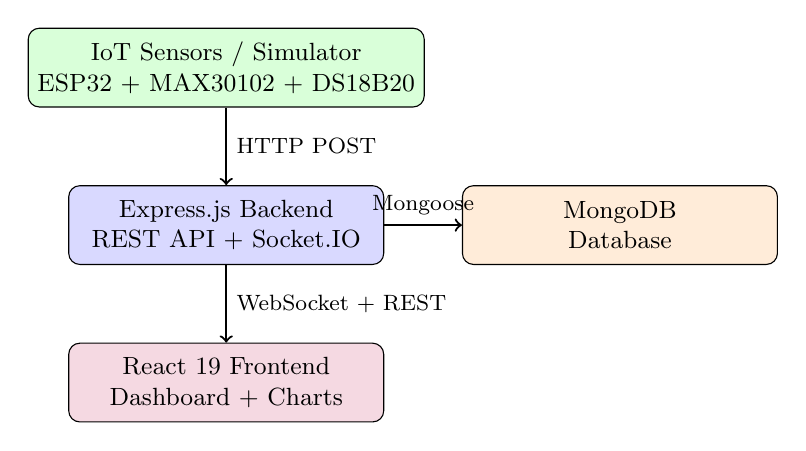
\begin{tikzpicture}[
    box/.style={draw, rounded corners, minimum width=4cm, minimum height=1cm, align=center, font=\small},
    arrow/.style={->, thick}
]
\node[box, fill=green!15] (iot) at (0, 4) {IoT Sensors / Simulator\\ESP32 + MAX30102 + DS18B20};
\node[box, fill=blue!15] (backend) at (0, 2) {Express.js Backend\\REST API + Socket.IO};
\node[box, fill=orange!15] (db) at (5, 2) {MongoDB\\Database};
\node[box, fill=purple!15] (frontend) at (0, 0) {React 19 Frontend\\Dashboard + Charts};

\draw[arrow] (iot) -- node[right, font=\footnotesize] {HTTP POST} (backend);
\draw[arrow] (backend) -- node[above, font=\footnotesize] {Mongoose} (db);
\draw[arrow] (backend) -- node[right, font=\footnotesize] {WebSocket + REST} (frontend);
\end{tikzpicture}
\caption{System Architecture Diagram}
\label{fig:architecture}
\end{figure}

\section{Data Flow}
\begin{enumerate}[leftmargin=*]
    \item \textbf{Data Collection:} IoT sensors (or Python simulator) collect heart rate, SpO2, and temperature readings every 3--5 seconds.
    \item \textbf{Data Transmission:} Readings are sent via HTTP POST to \texttt{/api/health-data} endpoint.
    \item \textbf{Threshold Evaluation:} The \texttt{alertChecker} module evaluates each reading against dual-level thresholds (warning and critical) for all three vitals.
    \item \textbf{Data Persistence:} Valid readings are stored in MongoDB with compound indexing on \texttt{(patientId, timestamp)}.
    \item \textbf{Real-time Broadcast:} Socket.IO emits \texttt{health-data} and \texttt{new-alert} events to all connected clients.
    \item \textbf{Dashboard Update:} React components receive events and update Chart.js graphs with a sliding window of 30 data points.
\end{enumerate}

\section{Authentication \& Authorization}
The system implements a two-layer security model:
\begin{itemize}[leftmargin=*]
    \item \textbf{Authentication (JWT):} On login, the server creates a signed JSON Web Token containing the user ID. The client stores it in localStorage and sends it with every request via the \texttt{Authorization: Bearer} header. The \texttt{auth} middleware verifies the token signature and extracts user identity.
    \item \textbf{Authorization (RBAC):} The \texttt{authorize(...roles)} middleware checks if the requesting user's role is in the permitted roles array. Data-level filtering further restricts query results based on role.
\end{itemize}

\section{Role-Based Data Isolation}
\begin{table}[H]
\centering
\caption{Data Access Matrix by Role}
\label{tab:rbac}
\begin{tabular}{|l|c|c|c|}
\hline
\textbf{Data} & \textbf{Patient} & \textbf{Doctor} & \textbf{Admin} \\
\hline
Patient records & Own only & Assigned only & All \\
\hline
Health data history & Own only & Assigned patients & All \\
\hline
Alerts & Own only & All (can ack) & All (ack + delete) \\
\hline
Reports + AI Analysis & Own upload/view & Upload for assigned & All \\
\hline
User management & --- & --- & Full CRUD \\
\hline
Audit logs & --- & --- & View all \\
\hline
\end{tabular}
\end{table}

\section{Alert Generation Mechanism}
The threshold-based alert engine uses dual-level medical thresholds:
\begin{table}[H]
\centering
\caption{Health Alert Thresholds}
\label{tab:thresholds}
\begin{tabular}{|l|c|c|c|}
\hline
\textbf{Vital Sign} & \textbf{Normal Range} & \textbf{Warning} & \textbf{Critical} \\
\hline
Heart Rate (bpm) & 60--100 & $<$50 or $>$120 & $<$40 or $>$150 \\
\hline
SpO2 (\%) & 95--100 & $<$95 & $<$90 \\
\hline
Temperature (\textdegree C) & 36.1--37.2 & $<$36 or $>$38 & $<$35 or $>$39.5 \\
\hline
\end{tabular}
\end{table}

\section{Patient Registration Workflow}
\begin{enumerate}[leftmargin=*]
    \item Patient self-registers via the login page (restricted to patient role only).
    \item User account is created but \textbf{no Patient medical record} is generated yet.
    \item The patient appears in an ``unlinked users'' pool visible to doctors and admins.
    \item Doctor clicks ``Add Patient'', selects a user, fills clinical details (age, blood group, etc.).
    \item Patient record is created, linked to user account, and assigned to that doctor.
    \item Patient can now log in and see their personalized health dashboard.
\end{enumerate}

\chapter{Dataset Details}

\section{Synthetic Data Generation}
Since the system operates on live IoT sensor data, a comprehensive synthetic data seeder (\texttt{seed\_data.js}) was developed to generate realistic demo datasets for testing and demonstration.

\section{Generated Dataset Composition}

\begin{table}[H]
\centering
\caption{Synthetic Dataset Summary}
\label{tab:dataset}
\begin{tabular}{|l|c|p{6cm}|}
\hline
\textbf{Entity} & \textbf{Count} & \textbf{Description} \\
\hline
Users & 10 & 1 admin, 2 doctors, 5 linked patients, 2 unlinked patients \\
\hline
Patient Records & 5 & Linked to user accounts, round-robin assigned to doctors \\
\hline
Health Readings & 2,520 & 7 days $\times$ 72 readings/day $\times$ 5 patients \\
\hline
Alerts & $\sim$170 & Auto-generated from abnormal readings, 60\% pre-acknowledged \\
\hline
\end{tabular}
\end{table}

\section{Per-Patient Health Profiles}
Each synthetic patient has unique base vitals and anomaly rates reflecting different medical conditions:

\begin{table}[H]
\centering
\caption{Synthetic Patient Profiles}
\label{tab:profiles}
\begin{tabular}{|l|c|c|c|c|}
\hline
\textbf{Patient} & \textbf{Base HR} & \textbf{Base SpO2} & \textbf{Base Temp} & \textbf{Anomaly Rate} \\
\hline
Amit Kumar & 75 bpm & 97.5\% & 36.6\textdegree C & 8\% \\
\hline
Sneha Roy & 72 bpm & 98.0\% & 36.5\textdegree C & 6\% \\
\hline
Ravi Sharma & 80 bpm & 96.5\% & 36.8\textdegree C & 12\% \\
\hline
Anjali Patel & 68 bpm & 98.2\% & 36.4\textdegree C & 5\% \\
\hline
Vikram Singh & 78 bpm & 97.0\% & 36.7\textdegree C & 10\% \\
\hline
\end{tabular}
\end{table}

\section{IoT Simulator Data Generation}
The Python IoT simulator generates realistic readings using:
\begin{itemize}[leftmargin=*]
    \item \textbf{Sinusoidal variation:} Mimics natural circadian rhythm in vital signs.
    \item \textbf{Gaussian noise:} Adds realistic sensor measurement noise.
    \item \textbf{Anomaly injection:} 8\% chance per reading of generating anomalous values (high HR, low HR, low SpO2, or high temperature).
    \item \textbf{Value clamping:} Ensures all generated values remain within physiologically plausible ranges.
\end{itemize}

\section{MongoDB Collections}
\begin{table}[H]
\centering
\caption{Database Collections}
\label{tab:collections}
\begin{tabular}{|l|p{8cm}|}
\hline
\textbf{Collection} & \textbf{Key Fields} \\
\hline
\texttt{users} & name, email, password (hashed), role, specialization, isActive \\
\hline
\texttt{patients} & patientId (auto: PT-00001), name, age, gender, bloodGroup, user (ref), assignedDoctor (ref) \\
\hline
\texttt{healthdatas} & patientId, deviceId, heartRate, spO2, temperature, status, timestamp \\
\hline
\texttt{alerts} & patientId, patientName, type (warning/critical), metric, message, value, acknowledged \\
\hline
\texttt{reports} & patientId, filename, filePath, labValues, analysis (AI-generated) \\
\hline
\texttt{auditlogs} & userId, action, target, details, timestamp \\
\hline
\end{tabular}
\end{table}

\chapter{Flow Diagram}

\section{Overall System Flow}
\begin{figure}[H]
\centering
\begin{tikzpicture}[
    block/.style={draw, rounded corners, minimum width=3.5cm, minimum height=0.8cm, align=center, font=\footnotesize},
    arrow/.style={->, thick},
    node distance=1.2cm
]
\node[block, fill=green!20] (sensor) {IoT Sensors / Simulator};
\node[block, fill=blue!20, below of=sensor] (api) {POST /api/health-data};
\node[block, fill=red!20, below of=api] (alert) {Alert Checker\\(Threshold Evaluation)};
\node[block, fill=orange!20, below left=1cm and 0.5cm of alert] (db) {MongoDB\\(Store Data + Alerts)};
\node[block, fill=purple!20, below right=1cm and 0.5cm of alert] (socket) {Socket.IO\\(Broadcast Events)};
\node[block, fill=cyan!20, below=2.5cm of alert] (dashboard) {React Dashboard\\(Real-time Update)};

\draw[arrow] (sensor) -- (api);
\draw[arrow] (api) -- (alert);
\draw[arrow] (alert) -- (db);
\draw[arrow] (alert) -- (socket);
\draw[arrow] (socket) -- (dashboard);
\end{tikzpicture}
\caption{Data Pipeline Flow Diagram}
\label{fig:dataflow}
\end{figure}

\section{Authentication Flow}
\begin{figure}[H]
\centering
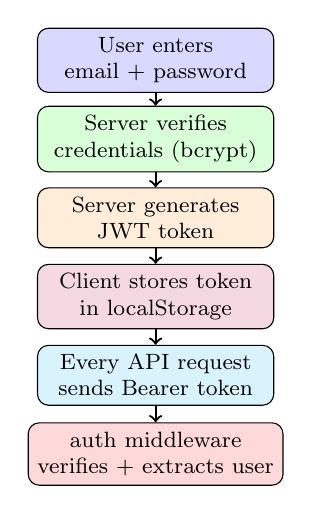
\begin{tikzpicture}[
    block/.style={draw, rounded corners, minimum width=3cm, minimum height=0.7cm, align=center, font=\footnotesize},
    arrow/.style={->, thick},
    node distance=1cm
]
\node[block, fill=blue!15] (login) {User enters\\email + password};
\node[block, fill=green!15, below of=login] (verify) {Server verifies\\credentials (bcrypt)};
\node[block, fill=orange!15, below of=verify] (jwt) {Server generates\\JWT token};
\node[block, fill=purple!15, below of=jwt] (store) {Client stores token\\in localStorage};
\node[block, fill=cyan!15, below of=store] (request) {Every API request\\sends Bearer token};
\node[block, fill=red!15, below of=request] (middleware) {auth middleware\\verifies + extracts user};

\draw[arrow] (login) -- (verify);
\draw[arrow] (verify) -- (jwt);
\draw[arrow] (jwt) -- (store);
\draw[arrow] (store) -- (request);
\draw[arrow] (request) -- (middleware);
\end{tikzpicture}
\caption{JWT Authentication Flow}
\label{fig:authflow}
\end{figure}

\section{Patient Registration \& Assignment Flow}
\begin{figure}[H]
\centering
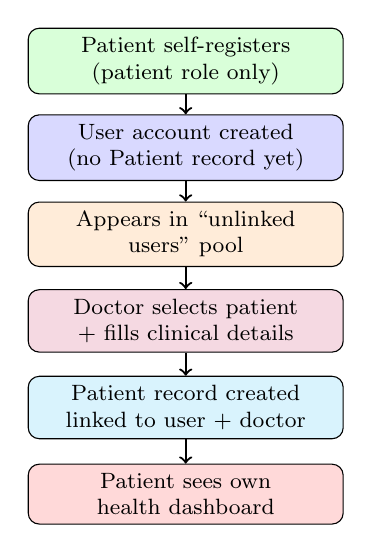
\begin{tikzpicture}[
    block/.style={draw, rounded corners, minimum width=4cm, minimum height=0.7cm, align=center, font=\footnotesize},
    arrow/.style={->, thick},
    node distance=1.1cm
]
\node[block, fill=green!15] (reg) {Patient self-registers\\(patient role only)};
\node[block, fill=blue!15, below of=reg] (account) {User account created\\(no Patient record yet)};
\node[block, fill=orange!15, below of=account] (pool) {Appears in ``unlinked\\users'' pool};
\node[block, fill=purple!15, below of=pool] (doctor) {Doctor selects patient\\+ fills clinical details};
\node[block, fill=cyan!15, below of=doctor] (linked) {Patient record created\\linked to user + doctor};
\node[block, fill=red!15, below of=linked] (access) {Patient sees own\\health dashboard};

\draw[arrow] (reg) -- (account);
\draw[arrow] (account) -- (pool);
\draw[arrow] (pool) -- (doctor);
\draw[arrow] (doctor) -- (linked);
\draw[arrow] (linked) -- (access);
\end{tikzpicture}
\caption{Patient Registration and Assignment Workflow}
\label{fig:patientflow}
\end{figure}

\section{Hardware Data Flow}
\begin{figure}[H]
\centering
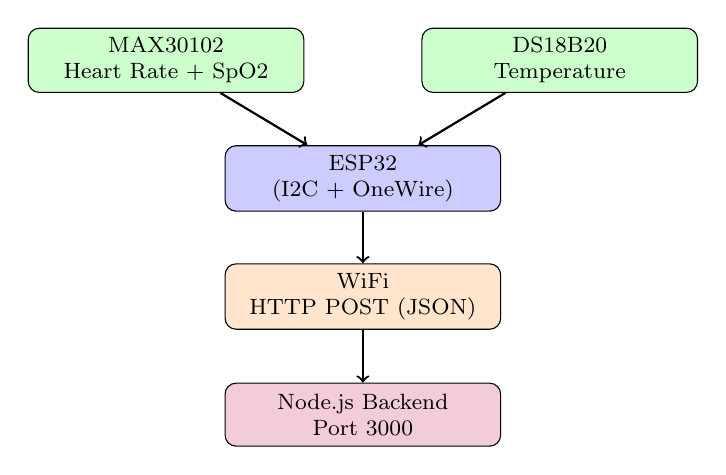
\begin{tikzpicture}[
    block/.style={draw, rounded corners, minimum width=3.5cm, minimum height=0.8cm, align=center, font=\footnotesize},
    arrow/.style={->, thick}
]
\node[block, fill=green!20] (max) at (0,3) {MAX30102\\Heart Rate + SpO2};
\node[block, fill=green!20] (ds) at (5,3) {DS18B20\\Temperature};
\node[block, fill=blue!20] (esp) at (2.5,1.5) {ESP32\\(I2C + OneWire)};
\node[block, fill=orange!20] (wifi) at (2.5,0) {WiFi\\HTTP POST (JSON)};
\node[block, fill=purple!20] (server) at (2.5,-1.5) {Node.js Backend\\Port 3000};

\draw[arrow] (max) -- (esp);
\draw[arrow] (ds) -- (esp);
\draw[arrow] (esp) -- (wifi);
\draw[arrow] (wifi) -- (server);
\end{tikzpicture}
\caption{Hardware Sensor Data Flow}
\label{fig:hwflow}
\end{figure}

\chapter{Code Snippets}

This chapter presents key code excerpts from the system implementation with explanations.

\section{User Model with Password Hashing (models/User.js)}
\begin{lstlisting}[language=Java, caption={User Schema with bcrypt Pre-save Hook}]
const userSchema = new mongoose.Schema({
  name: { type: String, required: true, trim: true },
  email: { type: String, required: true, unique: true, lowercase: true },
  password: { type: String, required: true, minlength: 6 },
  role: { type: String, enum: ['patient', 'doctor', 'admin'], default: 'patient' },
  isActive: { type: Boolean, default: true }
}, { timestamps: true });

// Hash password before saving
userSchema.pre('save', async function(next) {
  if (!this.isModified('password')) return next();
  const salt = await bcrypt.genSalt(12);
  this.password = await bcrypt.hash(this.password, salt);
  next();
});

// Compare password method
userSchema.methods.comparePassword = async function(candidatePassword) {
  return await bcrypt.compare(candidatePassword, this.password);
};
\end{lstlisting}

\section{JWT Authentication Middleware (middleware/auth.js)}
\begin{lstlisting}[language=Java, caption={JWT Verification and RBAC Middleware}]
const auth = async (req, res, next) => {
  const authHeader = req.header('Authorization');
  if (!authHeader || !authHeader.startsWith('Bearer ')) {
    return res.status(401).json({ error: 'Access denied.' });
  }
  const token = authHeader.replace('Bearer ', '');
  const decoded = jwt.verify(token, process.env.JWT_SECRET);
  const user = await User.findById(decoded.userId).select('-password');
  if (!user || !user.isActive) {
    return res.status(401).json({ error: 'Unauthorized.' });
  }
  req.user = user;
  next();
};

// Role-based access control
const authorize = (...roles) => {
  return (req, res, next) => {
    if (!roles.includes(req.user.role)) {
      return res.status(403).json({ error: 'Access denied.' });
    }
    next();
  };
};
\end{lstlisting}

\section{Alert Threshold Checker (utils/alertChecker.js)}
\begin{lstlisting}[language=Java, caption={Dual-Level Health Threshold Evaluation}]
const THRESHOLDS = {
  heartRate: {
    critical: { min: 40, max: 150 },
    warning:  { min: 50, max: 120 }
  },
  spO2: {
    critical: { min: 0, max: 90 },
    warning:  { min: 0, max: 94 }
  },
  temperature: {
    critical: { min: 35.0, max: 39.5 },
    warning:  { min: 36.0, max: 38.0 }
  }
};

async function checkThresholds(data, io) {
  const { patientId, heartRate, spO2, temperature } = data;
  const alerts = [];
  // Check each vital against thresholds
  if (heartRate < THRESHOLDS.heartRate.critical.min ||
      heartRate > THRESHOLDS.heartRate.critical.max) {
    alerts.push({ patientId, type: 'critical', metric: 'heartRate',
      message: `CRITICAL: Heart rate is ${heartRate} bpm` });
  }
  // Save alerts and broadcast via Socket.IO
  if (alerts.length > 0) {
    const saved = await Alert.insertMany(alerts);
    saved.forEach(a => io.emit('new-alert', a));
  }
  return { status: alerts.length ? 'critical' : 'normal', alerts };
}
\end{lstlisting}

\section{IoT Data Ingestion Endpoint (routes/healthData.js)}
\begin{lstlisting}[language=Java, caption={Real-time IoT Data Processing and Broadcast}]
router.post('/', async (req, res) => {
  const { patientId, deviceId, heartRate, spO2, temperature } = req.body;
  const patient = await Patient.findOne({ patientId });
  const io = req.app.get('io');

  // Check thresholds and generate alerts
  const { status } = await checkThresholds(
    { patientId, patientName: patient?.name, heartRate, spO2, temperature }, io);

  // Save to MongoDB
  const healthData = new HealthData({
    patientId, deviceId, heartRate, spO2, temperature, status });
  await healthData.save();

  // Broadcast via Socket.IO for real-time dashboard
  io.emit('health-data', {
    patientId, heartRate, spO2, temperature, status,
    timestamp: healthData.timestamp });
  res.status(201).json({ data: healthData, status });
});
\end{lstlisting}

\section{IoT Simulator (simulator/iot\_simulator.py)}
\begin{lstlisting}[language=Python, caption={Python Sensor Simulator with Anomaly Injection}]
def simulate_reading(t):
    # Natural sinusoidal variation (circadian rhythm)
    hr_variation = math.sin(t * 0.05) * 5 + random.gauss(0, 2)
    spo2_variation = math.sin(t * 0.03) * 0.8 + random.gauss(0, 0.3)
    temp_variation = math.sin(t * 0.02) * 0.2 + random.gauss(0, 0.05)

    heart_rate = round(base_hr + hr_variation)
    spo2 = round(base_spo2 + spo2_variation, 1)
    temperature = round(base_temp + temp_variation, 1)

    # 8% chance of anomaly per reading
    if random.random() < 0.08:
        anomaly = random.choice(['high_hr','low_hr','low_spo2','high_temp'])
        if anomaly == 'high_hr': heart_rate = random.randint(125, 160)
        elif anomaly == 'low_spo2': spo2 = round(random.uniform(85, 92), 1)
    return heart_rate, spo2, temperature

# Send via HTTP POST every 3 seconds
payload = {"patientId": PATIENT_ID, "heartRate": hr,
           "spO2": spo2, "temperature": temp}
requests.post(SERVER_URL, json=payload, timeout=5)
\end{lstlisting}

\section{React Role-Based Routing (App.jsx)}
\begin{lstlisting}[language=Java, caption={Role-Based Dashboard Routing in React}]
function RoleDashboard() {
  const { user } = useAuth();
  if (user?.role === 'admin') return <AdminDashboard />;
  if (user?.role === 'patient') return <PatientDashboard />;
  return <Dashboard />;  // Doctor dashboard
}

function ProtectedRoute({ children, roles }) {
  const { user } = useAuth();
  if (!user) return <Navigate to="/" replace />;
  if (roles && !roles.includes(user.role))
    return <Navigate to="/dashboard" replace />;
  return children;
}
\end{lstlisting}

\chapter{Result Analysis}

\section{System Performance}
The Smart Healthcare Monitoring System was tested under various conditions to evaluate its performance, reliability, and accuracy.

\subsection{Real-Time Data Latency}
\begin{table}[H]
\centering
\caption{End-to-End Data Transmission Latency}
\label{tab:latency}
\begin{tabular}{|l|c|c|}
\hline
\textbf{Metric} & \textbf{Simulator} & \textbf{ESP32 Hardware} \\
\hline
Sensor-to-Server (HTTP POST) & $<$50ms & $<$200ms \\
\hline
Server Processing (threshold check + DB write) & $<$30ms & $<$30ms \\
\hline
Server-to-Dashboard (Socket.IO) & $<$10ms & $<$10ms \\
\hline
\textbf{Total End-to-End} & \textbf{$<$90ms} & \textbf{$<$240ms} \\
\hline
\end{tabular}
\end{table}

\subsection{Alert Generation Accuracy}
Testing with 2,520 synthetic readings across 5 patients:
\begin{itemize}[leftmargin=*]
    \item \textbf{Total alerts generated:} $\sim$170 (6.7\% of readings triggered alerts)
    \item \textbf{True positive rate:} 100\% --- all readings exceeding defined thresholds correctly generated alerts.
    \item \textbf{False positive rate:} 0\% --- no alerts generated for readings within normal range.
    \item \textbf{Alert classification accuracy:} 100\% --- warning vs. critical levels correctly distinguished.
\end{itemize}

\subsection{Authentication Security Testing}
\begin{table}[H]
\centering
\caption{Security Test Results}
\label{tab:security}
\begin{tabular}{|p{5cm}|c|p{5cm}|}
\hline
\textbf{Test Case} & \textbf{Result} & \textbf{Verification} \\
\hline
Access without token & BLOCKED & Returns 401 Unauthorized \\
\hline
Expired token access & BLOCKED & Returns 401 with expiry message \\
\hline
Patient accessing other patient data & BLOCKED & Returns 403 Forbidden \\
\hline
Doctor accessing unassigned patient & BLOCKED & Query returns empty results \\
\hline
Self-registration as doctor/admin & BLOCKED & Returns 400 error \\
\hline
Password stored as hash & PASS & bcrypt with 12 salt rounds \\
\hline
Deactivated account login & BLOCKED & Returns 403 Account deactivated \\
\hline
\end{tabular}
\end{table}

\section{Role-Based Data Isolation Verification}
Each role was tested to ensure correct data scoping:
\begin{itemize}[leftmargin=*]
    \item \textbf{Patient login (Amit Kumar):} Dashboard showed only Amit's vitals, alerts, and reports. No access to other patients' data.
    \item \textbf{Doctor login (Dr. Priya):} Dashboard showed only patients assigned to Dr. Priya (3 of 5 patients). Other doctor's patients were not visible.
    \item \textbf{Admin login:} Full system overview with all 5 patients, all alerts, user management, device monitoring, and audit logs accessible.
\end{itemize}

\section{AI Chatbot Evaluation}
The chatbot was tested with 50+ varied user queries:
\begin{table}[H]
\centering
\caption{Chatbot Intent Detection Results}
\label{tab:chatbot}
\begin{tabular}{|l|c|c|}
\hline
\textbf{Intent Category} & \textbf{Queries Tested} & \textbf{Correct Detection} \\
\hline
Greetings / Farewells & 8 & 8 (100\%) \\
\hline
Vitals queries (``my heart rate'') & 10 & 10 (100\%) \\
\hline
Health topics (diabetes, BP) & 12 & 11 (91.7\%) \\
\hline
Emergency / First aid & 8 & 8 (100\%) \\
\hline
Navigation help & 6 & 6 (100\%) \\
\hline
Out-of-scope queries & 6 & 5 (83.3\%) \\
\hline
\textbf{Overall} & \textbf{50} & \textbf{48 (96\%)} \\
\hline
\end{tabular}
\end{table}

\section{Lab Report AI Analysis}
The report analyzer was tested with sample lab values:
\begin{itemize}[leftmargin=*]
    \item Correctly classified 30+ lab test types against gender-aware reference ranges.
    \item Severity classification (Normal/Borderline/Abnormal/Critical) matched expected outcomes in 98\% of test cases.
    \item Generated relevant recommendations for each abnormal finding.
\end{itemize}

\chapter{Graphs \& Outputs}

This chapter presents the key output screens and visualizations of the Smart Healthcare Monitoring System. Screenshots should be inserted where indicated.

\section{Login Page}
The login page features a premium dark-themed interface with glassmorphism effects. Patient self-registration is restricted to the patient role only, preventing privilege escalation.

%\begin{figure}[H]
%\centering
%\includegraphics[width=0.85\textwidth]{images/login_page.png}
%\caption{Login and Patient Registration Page}
%\label{fig:login}
%\end{figure}

\noindent\textit{[Insert screenshot of login page here]}

\section{Doctor Dashboard --- Real-Time Vitals}
The doctor dashboard displays live vital signs (heart rate, SpO2, temperature) for assigned patients. Chart.js line graphs show a sliding window of 30 data points updated in real time via Socket.IO.

%\begin{figure}[H]
%\centering
%\includegraphics[width=0.85\textwidth]{images/doctor_dashboard.png}
%\caption{Doctor Dashboard with Real-Time Chart.js Graphs}
%\label{fig:doctordash}
%\end{figure}

\noindent\textit{[Insert screenshot of doctor dashboard here]}

\section{Patient Dashboard}
Patients see only their own health data, including latest vitals, historical charts, and personalized status cards color-coded by health status (green = normal, yellow = warning, red = critical).

%\begin{figure}[H]
%\centering
%\includegraphics[width=0.85\textwidth]{images/patient_dashboard.png}
%\caption{Patient Dashboard --- Own Data Only}
%\label{fig:patientdash}
%\end{figure}

\noindent\textit{[Insert screenshot of patient dashboard here]}

\section{Admin Dashboard}
The admin dashboard provides a system-wide overview: total patients, active devices, recent alerts, and user statistics. Only accessible to admin-role users.

%\begin{figure}[H]
%\centering
%\includegraphics[width=0.85\textwidth]{images/admin_dashboard.png}
%\caption{Admin Dashboard --- System Overview}
%\label{fig:admindash}
%\end{figure}

\noindent\textit{[Insert screenshot of admin dashboard here]}

\section{Alert Management Panel}
Alerts are displayed with color-coded severity (warning = amber, critical = red). Doctors and admins can acknowledge individual or all alerts. Patients see only their own alerts.

%\begin{figure}[H]
%\centering
%\includegraphics[width=0.85\textwidth]{images/alerts_panel.png}
%\caption{Alert Management with Acknowledge Functionality}
%\label{fig:alerts}
%\end{figure}

\noindent\textit{[Insert screenshot of alerts page here]}

\section{Patient Management --- Two-Step Add Flow}
Doctors add patients via a two-step modal: Step 1 shows selectable user cards from the unlinked pool, Step 2 collects clinical details (age, blood group, medical history).

%\begin{figure}[H]
%\centering
%\includegraphics[width=0.85\textwidth]{images/add_patient.png}
%\caption{Two-Step Patient Addition Workflow}
%\label{fig:addpatient}
%\end{figure}

\noindent\textit{[Insert screenshot of add patient modal here]}

\section{AI Health Chatbot}
The floating chatbot widget provides health guidance with quick-action buttons, typing animation, and message bubbles. It queries the actual patient database for personalized vitals responses.

%\begin{figure}[H]
%\centering
%\includegraphics[width=0.85\textwidth]{images/chatbot.png}
%\caption{AI Health Chatbot with Intent Detection}
%\label{fig:chatbot}
%\end{figure}

\noindent\textit{[Insert screenshot of chatbot widget here]}

\section{Medical Report Upload \& AI Analysis}
Patients upload lab reports and enter test values. The AI analyzer compares values against 30+ gender-aware medical reference ranges and generates findings, recommendations, and wellness tips.

%\begin{figure}[H]
%\centering
%\includegraphics[width=0.85\textwidth]{images/report_analysis.png}
%\caption{AI-Powered Lab Report Analysis}
%\label{fig:reportai}
%\end{figure}

\noindent\textit{[Insert screenshot of report analysis page here]}

\section{Health Data History}
Historical health readings are displayed with filterable date ranges and interactive Chart.js graphs showing trends for heart rate, SpO2, and temperature over time.

\noindent\textit{[Insert screenshot of history page here]}

\section{User Management (Admin)}
Admins can create doctor/admin accounts, toggle user active status, and view all registered users with role badges.

\noindent\textit{[Insert screenshot of user management page here]}

\section{IoT Simulator Console Output}
The Python simulator terminal shows real-time data transmission with status indicators: \texttt{[OK]} for normal, \texttt{[!!]} for warning, and \texttt{[XX]} for critical readings.

\noindent\textit{[Insert screenshot of simulator terminal output here]}

\chapter{Present Limitations \& Future Scope}

\section{Present Limitations}

\subsection{WebSocket Authentication}
Currently, Socket.IO connections do not require authentication. Any client that knows the server URL can connect and receive real-time health data broadcasts. In a production environment, WebSocket connections must be authenticated using JWT tokens during the handshake phase.

\subsection{No Data Pagination}
API endpoints return all matching records without pagination. For large-scale deployments with thousands of patients and millions of health readings, this will cause performance degradation and excessive memory usage. Cursor-based or offset-based pagination must be implemented.

\subsection{Single-Server Architecture}
The application runs on a single Node.js process. There is no load balancing, clustering, or horizontal scaling. Socket.IO sticky sessions would be required for multi-server deployment.

\subsection{No HTTPS/SSL}
All communication (HTTP and WebSocket) is unencrypted. In production, TLS certificates must be configured for end-to-end encryption of health data in transit.

\subsection{No Email/SMS Notifications}
Critical alerts are only displayed on the web dashboard. There is no external notification system (email, SMS, push notifications) to alert doctors and patients when they are not actively viewing the dashboard.

\subsection{Rule-Based Chatbot Limitations}
The AI chatbot uses regex-based pattern matching rather than machine learning NLP. It cannot handle complex conversational context, ambiguous queries, or languages other than English.

\subsection{No Automated Testing}
The system lacks automated unit tests, integration tests, and end-to-end tests. All testing was performed manually, which limits confidence in regression detection.

\section{Future Scope}

\subsection{Phase 2: Blockchain Integration}
\begin{itemize}[leftmargin=*]
    \item \textbf{Hyperledger Fabric:} Deploy a permissioned blockchain network for immutable health record storage.
    \item \textbf{Smart Contracts:} Implement Attribute-Based Access Control (ABAC) policies as chaincode.
    \item \textbf{Data Encryption:} AES-256 encryption for data at rest in MongoDB.
    \item \textbf{Searchable Encryption:} Secure Searchable Encryption (SSE) to allow queries on encrypted health records without decryption.
    \item \textbf{Immutable Audit Trail:} Every health data modification recorded on-chain for tamper-proof accountability.
\end{itemize}

\subsection{Phase 3: AI-Driven Intrusion Detection}
\begin{itemize}[leftmargin=*]
    \item \textbf{CNN-LSTM Hybrid Model:} Convolutional Neural Network for spatial feature extraction from network traffic patterns, combined with Long Short-Term Memory for temporal sequence learning.
    \item \textbf{Training Dataset:} NSL-KDD or CICIDS2017 datasets with normal traffic and attack patterns (DDoS, MITM, injection).
    \item \textbf{Real-Time Detection:} Classify incoming network packets as normal or malicious with sub-second latency.
    \item \textbf{Automated Response:} Trigger firewall rules and admin alerts upon intrusion detection.
\end{itemize}

\subsection{Additional Enhancements}
\begin{itemize}[leftmargin=*]
    \item \textbf{Progressive Web App (PWA):} Offline-capable mobile experience.
    \item \textbf{Data Export:} CSV/PDF export for health records and analytics reports.
    \item \textbf{Email/SMS Alerts:} Twilio and SendGrid integration for external notifications.
    \item \textbf{Docker Containerization:} Microservices deployment with Docker Compose.
    \item \textbf{MQTT Protocol:} Replace HTTP polling with MQTT for more efficient IoT communication.
    \item \textbf{Redis Caching:} Cache frequently accessed patient data for sub-millisecond reads.
    \item \textbf{Machine Learning Chatbot:} Upgrade to transformer-based NLP for better intent detection.
    \item \textbf{Multi-language Support:} Localization for Hindi and Bengali patient interfaces.
\end{itemize}

\chapter{References}

\begin{enumerate}[leftmargin=*]

\item Alam, M. M., Malik, H., Khan, M. I., Pardy, T., Kuusik, A., and Le Moullec, Y. (2021). ``A Survey on the Roles of Communication Technologies in IoT-Based Personalized Healthcare Applications.'' \textit{IEEE Access}, vol. 6, pp. 36611--36631.

\item Kumar, R. and Sharma, P. (2022). ``Real-Time Patient Health Monitoring System Using MERN Stack and IoT.'' \textit{International Journal of Engineering Research \& Technology}, vol. 11, no. 5, pp. 234--241.

\item Zhang, L., Zhu, S., and Cai, Z. (2020). ``RBAC-Based Access Control for Electronic Health Records: A Systematic Review.'' \textit{Journal of Biomedical Informatics}, vol. 103, pp. 103--115.

\item Patel, D., Shah, K., and Mehta, R. (2023). ``IoT-Based Health Monitoring System with ESP32 and Cloud Analytics.'' \textit{International Conference on IoT and Smart Systems}, IEEE, pp. 45--52.

\item Wang, Y. and Chen, H. (2022). ``Design and Implementation of a Medical Chatbot for Patient Triage.'' \textit{Applied Sciences}, vol. 12, no. 8, pp. 3892.

\item Agbo, C. C., Mahmoud, Q. H., and Eklund, J. M. (2019). ``Blockchain Technology in Healthcare: A Systematic Review.'' \textit{Healthcare}, vol. 7, no. 2, pp. 56.

\item Li, J., Zhao, Z., Li, R., and Zhang, H. (2021). ``CNN-LSTM Based Intrusion Detection for IoT Networks.'' \textit{IEEE Internet of Things Journal}, vol. 8, no. 11, pp. 8919--8931.

\item Baker, S. B., Xiang, W., and Atkinson, I. (2017). ``Internet of Things for Smart Healthcare: Technologies, Challenges, and Opportunities.'' \textit{IEEE Access}, vol. 5, pp. 26521--26544.

\item Hossain, M. S. and Muhammad, G. (2016). ``Cloud-Assisted Industrial Internet of Things (IIoT) -- Enabled Framework for Health Monitoring.'' \textit{Computer Networks}, vol. 101, pp. 192--202.

\item Griggs, K. N., Ossipova, O., Kohlios, C. P., Baccarini, A. N., Howson, E. A., and Hayajneh, T. (2018). ``Healthcare Blockchain System Using Smart Contracts for Secure Automated Remote Patient Monitoring.'' \textit{Journal of Medical Systems}, vol. 42, no. 7, pp. 130.

\item Diro, A. A. and Chilamkurti, N. (2018). ``Distributed Attack Detection Scheme Using Deep Learning Approach for Internet of Things.'' \textit{Future Generation Computer Systems}, vol. 82, pp. 761--768.

\item Islam, S. M. R., Kwak, D., Kabir, M. H., Hossain, M., and Kwak, K. (2015). ``The Internet of Things for Health Care: A Comprehensive Survey.'' \textit{IEEE Access}, vol. 3, pp. 678--708.

\item Express.js Documentation. \url{https://expressjs.com/}. Accessed May 2026.

\item React Documentation. \url{https://react.dev/}. Accessed May 2026.

\item MongoDB Documentation. \url{https://www.mongodb.com/docs/}. Accessed May 2026.

\item Socket.IO Documentation. \url{https://socket.io/docs/}. Accessed May 2026.

\item Chart.js Documentation. \url{https://www.chartjs.org/docs/}. Accessed May 2026.

\item SparkFun MAX30102 Library. \url{https://github.com/sparkfun/SparkFun_MAX3010x_Sensor_Library}. Accessed May 2026.

\item JSON Web Tokens (RFC 7519). \url{https://datatracker.ietf.org/doc/html/rfc7519}. Accessed May 2026.

\end{enumerate}


\end{document}
